% Thanks to Seth Johnson (sethrj@umich.edu) for publishing his ans template

%%%%%%%%%%%%%%%%%%%%%%%%%%%%%%%%%%%
\documentclass{anstrans}
\bibliographystyle{ans}

%%%%%%%%%%%%%%%%%%%%%%%%%%%%%%%%%%%
\title{Once-Through Benchmarks with \textsc{Cyclus}, a Modular, Open-Source Fuel Cycle Simulator}
\author{Matthew J.~Gidden, Paul P.H.~Wilson, Kathryn D.~Huff, Robert W.~Carlsen}
\institute{Department of Nuclear Engineering \& Engineering Physics, University of Wisconsin - Madison, Madison, WI, 53703}
\email{gidden@wisc.edu}
\date{2012/06/29}

%%%%%%%%%%%%%%%%%%%%%%%%%%%%%%%%%%%
\usepackage{times} % fancier looking type
\usepackage{graphicx}
\usepackage{microtype} % if using PDF
\usepackage{amsmath} % for optimization equations
\usepackage{booktabs}

%%%%%%%%%%%%%%%%%%%%%%%%%%%%%%%%%%%
\begin{document}

%%%%%%%%%%%%%%%%%%%%%%%%%%%%%%%%%%%%%%%%%%%%%%%%%%%%%%%%%%%%%%%%%%%%%%%%%%%%%%%%
\section{Introduction}
The \textsc{Cyclus} project, based at the University of Wisconsin -
Madison, is an open source platform for exploring the long-term impact
of alternative nuclear fuel cycles.  The \textsc{Cyclus} core provides
the infrastructure for an agent-based approach, allowing user-provided
modules to define the behavior of fuel cycle facilities as they
interact to exchange materials.  An important consequence of this
approach is that innovative facility and material exchange concepts
can be introduced to a consistent framework allowing for more rigorous
comparison.  The \textsc{Cyclus} team has recently grown and now
incorporates a variety of expertise: output visualization capability
through collaboration with the University of Utah, server-client
communication via the University of Idaho, input visualization and
control with the University of Texas - Austin, and social
communication expertise through collaborators at UW-Madison to assist
the mission-critical goal of relevancy vis-\`{a}-vis policy
makers. Accordingly, the \textsc{Cyclus} project is expanding efforts in
the realms of both structural capability and benchmarking
calculations.

A series of once-through fuel cycle scenarios are being conducted
using the \textsc{Cyclus} core and accompanying modules. Where needed,
additional modules have been added, including a region model that intelligently makes building decisions 
given a demand function. The results of these scenarios are then compared with
VISION~\cite{vision2009} to provide a benchmark of the \textsc{Cyclus}
results.

%%%%%%%%%%%%%%%%%%%%%%%%%%%%%%%%%%%%%%%%%%%%%%%%%%%%%%%%%%%%%%%%%%%%%%%%%%%%%%%%
\section{\textsc{Cyclus} Design and Development}
The paradigm under which \textsc{Cyclus} has been developed and is
distributed is unique and offers a number of advantages regarding its
potential wide-spread adoption by a diverse user base. \textsc{Cyclus}
is an open source collection of libraries that provides
out-of-the-box capability as well as a platform on which to develop
additional modules. At present, the \textsc{Cyclus} suite includes a
core library, a module development toolkit, and a basic module pack.
The module development toolkit includes a growing collection of
standard and commonly used capabilities, such as an interface to optimization 
problem solvers and resource buffers for storing inventories.

%%%%%%%%%%
\subsection{Open Development}
As one of the leading principles guiding the development of
\textsc{Cyclus}, an open-source repository provides a high degree of
flexibility and a large amount of exposure to potential collaborators
and developers. The \textsc{Cyclus} repository is publicly available via
GitHub~\cite{cyclus2012}. A number of tools are available to
\textsc{Cyclus} developers in order to maintain software development
best-practices, including distributed version control, automatic
documentation, and in-depth issue management. Additionally,
\textsc{Cyclus} developers have taken advantage of existing, external
open-source libraries in order to conform to current standards,
including an expansion of the C++ standard library and fully
benchmarked linear and integer programming solvers. Perhaps the most
important attribute of the open development paradigm is that it allows
for unfettered access to the \textsc{Cyclus} core and basic module
source code. Combined with modular software development, \textsc{Cyclus}
is an easily transferable framework on which to build a strong fuel
cycle simulation community.

%%%%%%%%%%
\subsection{Dynamic Module Capability}
Incorporation of dynamically loadable, independently constructed
modules is another key design concept in \textsc{Cyclus}. Whereas the
connections between staticly loaded libraries is determined at compile time,
dynamically loaded libraries are linked at run time. This allows for the core
simulation engine comprising \textsc{Cyclus} to be physically separate from
the various modules determining the specific behavior that occurs in
each simulation.  Because interaction between the core and modules occurs via
dynamic linking, module development is encapsulated and can be performed without involving
the simulation engine, increasing efficiency and decreasing the
overall programming experience required. This separation
not only allows for multiple developers to work towards a common goal,
e.g. fully describing a target scenario, but also assists in
separating simulation concerns into reasonably sized, independently
testable modules.

%%%%%%%%%%
\subsection{Optimization}
The \textsc{Cyclus} project has recently added a linear, integer, and
mixed integer program wrapper named \textsc{Cyclopts}~\cite{cyclopts2012} to
its tool set. \textsc{Cyclopts} relies on the open-source solver Coin-OR Branch
and Cut~\cite{coinCBC}, providing a simple interface to describe such
optimization problems. At the present time, developers have the
ability to define a set of variables and to describe an objective
function and series of constraints that utilize some subset of those
variables. Variables currently come in two flavors, integer and
linear, corresponding to their respective solution
techniques. Additional work will be performed to add cutting plane
support as well as a suite of unit tests.

%%%%%%%%%%%%%%%%%%%%%%%%%%%%%%%%%%%%%%%%%%%%%%%%%%%%%%%%%%%%%%%%%%%%%%%%%%%%%%%%
\section{Verification and Testing}

%%%%%%%%%%
\subsection{Core Functionality Benchmarks}
To verify the functionality of the \textsc{Cyclus} core, basic problems using a 
single reactor type were performed and compared to results from both VISION and 
GENIUS~\cite{juchau2008}, another fuel cycle simulator and predecessor to 
\textsc{Cyclus}. Table~\ref{tab:scenarioparams} describes the parameters varied 
in the functionality benchmark.
%%%
\begin{table} [h]
\centering
\begin{tabular} {|c|c|c|} 
\hline
Problem No. & No.Reactors & Growth Type \\
\hline
1           & 1          & none        \\
2           & 10         & none        \\
3           & 1          & linear      \\
4           & 1          & exponential \\
\hline
\end{tabular}
  \caption{Core Functionality Benchmarking Parameters.}
  \label{tab:scenarioparams}
\end{table}
%%%

%%%%%%%%%%
\subsection{Once-Through Fuel Cycle Benchmarks}
Once-through simulation results were compared with similarly defined
scenarios in VISION.  For \textsc{Cyclus}, a subset of real-world facilities
and their interactions were included: mines, enrichment facilities, reactors,
and storage facilities. In order to drive the simulation, an
electricity demand function is provided to the simulation, which
determines the supply requirement for reactors at a given time
step. Once the simulation is complete, an analysis of material flows
and facility deployment as a function of time is provided. Of specific
concern with respect to the once-through fuel cycle is long term used
fuel production and the corresponding storage requirements.

%%%%%%%%%%
\subsubsection{Scenario Construction}
Reactor deployment decisions are driven by the region in which the 
reactors exist. An electricity demand is defined for that region, either as a
linear or exponential function. The region is also provided with a set
of available facilities (reactors) that can meet this demand. At any time step
in which there exists a demand gap, i.e. there exists more demand than
supply, a build decision is made. This decision is modeled as the
following integer program:
%%%
\begin{subequations} \label{eqs:optBuild}
\begin{equation} \label{eq:optBuildObj}
\begin{aligned}
& \min
& & \sum_{i \in I}n_i*c_i
\end{aligned}
\end{equation}
\begin{equation} \label{eq:optBuildConst}
\begin{aligned}
& \text{s.t.}
& & \sum_{i \in I}n_i*\phi_i \ge \Phi
\end{aligned}
\end{equation}
\begin{equation} \label{eq:optBuildBounds}
\begin{aligned}
& n_i \in [0,\infty) & \forall \:\: i \in I &
\end{aligned}
\end{equation}
\begin{equation} \label{eq:optBuildInt}
\begin{aligned}
& n_i \:\:\: integer & \forall \:\: i \in I &
\end{aligned}
\end{equation}
where $\Phi$ is the unmet demand, $I$ is the set of facilities capable of 
meeting the demand, and, for each facility in $I$, $c_i$ is the cost of building, 
and $\phi_i$ is the nameplate capacity.  Finally, $n_i$ is the optimized number of
facilities to build of type $i$.
\end{subequations}
%%%

While electricity demand directly corresponds to reactor deployment,
supporting facilities, e.g. enrichment facilities, mines, and storage
facilities, depend on overall reactor fuel input and output
requirements. There are multiple strategies that can be used to
determine supporting facility deployment, of which a minimal
constraint approach is first analyzed followed by a supply-demand
constraint approach, i.e. when the demand for a resource, e.g. fresh
fuel, reaches a percentage of the total supply, a facility meeting
that demand is deployed.

%%%%%%%%%%
\subsubsection{Benchmarking and Parameter Variation}
VISION uses an Excel spreadsheet input paradigm which allows one to
develop new scenarios or vary the parameters of the provided ``Base
Case Scenarios''. The once-through base case scenario is used and some
of its corresponding parameters are varied in order to define a
relative benchmark between \textsc{Cyclus} and VISION. Specifically, the
following parameters are varied:
\begin{itemize}
\item number of reactor types (e.g. LWRs and HWRs)
\item electricity demand rate
\item storage availability date (i.e. when a repository is available)
\end{itemize}

%%%%%%%%%%%%%%%%%%%%%%%%%%%%%%%%%%
\section{Results \& Conclusions}

%%%%%%%%%%
\subsubsection{Results}
\textsc{Cyclus} has performed well in early verification comparisons with VISION.
Results of the core functionality benchmark problems, which report total mass 
ejected from reactors as a function of time, are shown below in Fig.~\ref{fig:p1} 
and Fig.~\ref{fig:p2}; note that the benchmark values used for VISION and GENIUS have 
been previously reported in Oliver2009~\cite{oliver2009}.
\begin{figure}[ht]
  \centering
  \includegraphics[width=0.48\textwidth]{p1.ps}
  \caption{Results from Problem 1.}
  \label{fig:p1}
\end{figure}
\begin{figure}[ht]
  \centering
  \includegraphics[width=0.48\textwidth]{p2.ps}
  \caption{Results from Problem 2.}
  \label{fig:p2}
\end{figure}

A fundamental and expected result from this work is the effect of continuous
material flow simulators, such as VISION, versus the discrete nature of 
GENIUS and \textsc{Cyclus}. This difference accounts for the small discrepancies
during the final core offload(s)~\cite{oliver2009}.

%%%%%%%%%%
\subsubsection{Conclusions}
The \textsc{Cyclus} core has been shown to provide expected behavior of discrete 
material flows for simple reactor cases. \textsc{Cyclus} additionally has the 
capability not only to model a variety of growth scenarios with varying fuel storage 
strategies, but also to emulate the reactor deployment algorithm of VISION, i.e. 
explicitly declaring reactor types to be built given a defined distribution, by adding 
an additional constraint in the decision making problem solved by the region in
which the reactors exist.

Further work is currently underway to refine building strategies for
non-reactor facilities; however, the next major project goal of the
\textsc{Cyclus} team is to provide recycle capability. Once completed,
additional benchmarks will be performed to analyze code behavior using
recycle scenarios.

%%%%%%%%%%%%%%%%%%%%%%%%%%%%%%%%%%%%%%%%%%%%%%%%%%%%%%%%%%%%%%%%%%%%%%%%%%%%%%%%
\section{Acknowledgments}
This research is being performed using funding received from the DOE
Office of Nuclear Energy's Nuclear Energy University Programs.  The
author thanks the NEUP for its generous support.

%%%%%%%%%%%%%%%%%%%%%%%%%%%%%%%%%%%%%%%%%%%%%%%%%%%%%%%%%%%%%%%%%%%%%%%%%%%%%%%%
\bibliography{bibliography}
\end{document}
